\documentclass[xcolor=table]{beamer}

% Use Packages
%
\usepackage{booktabs}
\usepackage{hyperref}
%\usepackage[acronym,toc]{glossaries} %%%% Acronym/glossary support
\usepackage[style=tree,numberedsection]{glossaries-extra}
\usepackage[flushleft]{threeparttable}
\usepackage{cite}
\usepackage{soul}
\usepackage{xr}
\usepackage{xspace}
\usepackage{subfig}
\usepackage{nuc}
\usepackage{multirow}

\loadglsentries{acros}

\newcommand{\Cyclus}{\textsc{Cyclus}\xspace}
\newcommand{\Cycamore}{\textsc{Cycamore}\xspace}
\newcommand{\Trailmap}{\textsc{Trailmap}\xspace}

\author{Buckingham U. Badger}
\institute{Preliminary examination for the\\ degree of Doctor of Philosophy,\\ Nuclear Engineering and Engineering Physics}

\date{DATE} 
\title{Lorem Ipsum nunc sed id semper risus in hendrerit}

\AtBeginSection[]
{
    \begin{frame}
        \frametitle{Table of Contents}
        \tableofcontents[currentsection,
        currentsubsection,
        subsectionstyle=show/show/shaded,
        subsubsectionstyle=hide/hide/hide] %show = current subsection is shown regularly, shaded = the section's other subsections are shown, but shaded, hide = other sections' subsection entries are not shown in the table of contents
    \end{frame}
}

% [white] is standard theme
% [compactlogo] refers to the use of the wide rather than tall logo on the title page
% [cnerglogo] places the CNERG logo next to the UW crest on content slides. Remove for UW only logo. Use [cnergonlylogo] to only have CNERG logo and not UW logo
\usetheme[white,compactlogo,cnerglogo]{Wisconsin}

\begin{document}
\newcommand*{\alphabet}{ABCDEFGHIJKLMNOPQRSTUVWXYZabcdefghijklmnopqrstuvwxyz}
\newlength{\highlightheight}
\newlength{\highlightdepth}
\newlength{\highlightmargin}
\setlength{\highlightmargin}{2pt}
\settoheight{\highlightheight}{\alphabet}
\settodepth{\highlightdepth}{\alphabet}
\addtolength{\highlightheight}{\highlightmargin}
\addtolength{\highlightdepth}{\highlightmargin}
\addtolength{\highlightheight}{\highlightdepth}
\newcommand*{\Highlight}{\rlap{\textcolor{HighlightBackground}{\rule[-\highlightdepth]{\linewidth}{\highlightheight}}}}

%turn off fancy headline for title page
\setbeamertemplate{headline}{}
\setbeamertemplate{footline}{}
  
\begin{frame}
\vspace{-25pt}
\titlepage
\end{frame}

%turn on fancy headline for rest of slides
\setbeamertemplate{bibliography item}{\insertbiblabel}
\setbeamertemplate{navigation symbols}{}

\setbeamertemplate{headline}
{%
  \begin{beamercolorbox}{section in head/foot}
    \vskip2pt\insertnavigation{\paperwidth}\vskip2pt
  \end{beamercolorbox}%
  \begin{beamercolorbox}[colsep=1pt]{lower fine separation line head}
  \end{beamercolorbox}
}

\defbeamertemplate*{footline}{subtle theme}
{
  \leavevmode%
  \makebox[\paperwidth][r]{\insertframenumber{} / \inserttotalframenumber{}\hspace*{1ex}}%
  \vspace*{1ex}%
  \vskip0pt%
}

%% Slides
\begin{frame}{Objective}
\centering
    \Large To develop tools and methods that enhance
    
     \textbf{[a particular thing]} 
     
     as a means to improve 
    
    \textbf{[some metric]}
    
    of [subfield of nuclear engineering]
\end{frame}

\begin{frame}
\frametitle{Table of Contents}
\tableofcontents[subsubsectionstyle=hide]
\end{frame}

\section{Introduction}

\subsection{Viverra suspendisse}

% ---------------------------------------------- %
\begin{frame}{Lorem ipsum dolor sit amet}
\vspace{-12pt}
\begin{columns}
\column{0.65\textwidth}
\begin{itemize}
    \item consectetur adipiscing elit
    \begin{itemize}
        \item sed do eiusmod tempor incididunt
        \item ut labore et dolore magna aliqua
        \item Ut enim ad minim veniam
    \end{itemize}
    \bigskip 
    \item Sed id semper risus in hendrerit gravida rutrum quisque non\cite{knox_ratio_2012}
    \bigskip 
    \item A scelerisque purus semper eget duis at tellus. 
    \item quis nostrud exercitation ullamco laboris nisi ut aliquip ex ea commodo consequat\cite{xie_youwont_2023,weiherer_zero_2023}
\end{itemize}
\column{0.35\textwidth}
\begin{figure}
    \centering
    
\includegraphics[width=\linewidth]{images/BuckyBadger.png}
    \label{fig:cyclus_ecosystem}
\end{figure}
\end{columns}
\end{frame}
% ---------------------------------------------- %

\subsection{Potenti nullam ac tortor vitae}

% ---------------------------------------------- %
\begin{frame}{Duis aute irure}
    \begin{itemize}
        \item At erat pellentesque adipiscing commodo\cite{gato_schroedingers_2011}. Non arcu risus quis varius quam quisque. Adipiscing bibendum est ultricies integer quis auctor elit sed\cite{mathieu_fun_2022}. Egestas pretium aenean pharetra magna ac placerat vestibulum. 
        \bigskip
        \item dolor in reprehenderit in voluptate velit esse cillum dolore eu fugiat nulla pariatur
        \begin{itemize}
            \item Excepteur sint occaecat cupidatat non proident
            \item sunt in culpa qui officia deserunt
            \item mollit anim id est laborum
        \end{itemize}
    \end{itemize}
\end{frame}
% ---------------------------------------------- %


% ---------------------------------------------- %
\begin{frame}{Varius morbi enim nunc faucibus.}
    \begin{itemize}
    \item Nam at lectus urna duis convallis.
    \begin{itemize}
        \item Porta lorem mollis aliquam ut porttitor leo a diam. Vitae auctor eu augue ut lectus arcu bibendum at varius. Enim ut tellus elementum sagittis vitae et\cite{polishchuk_gender-aware_2018}. Nibh sed pulvinar proin gravida hendrerit lectus a. Nisl suscipit adipiscing bibendum est ultricies integer quis.
        \item Orci porta \textbf{\alert{non pulvinar}}
    \end{itemize}
    \item Proin fermentum leo vel orci porta non. Suspendisse interdum consectetur libero id faucibus nisl. 
    \end{itemize}
    \bigskip
    $\therefore$ Vitae justo eget \textbf{magna} fermentum iaculis eu. Ullamcorper a lacus \textbf{vestibulum} sed arcu non \textbf{odio} euismod lacinia.
\end{frame}
% ---------------------------------------------- %

\section{Lit Review}

%\subsection{Nonproliferation applications of FCS}

% ---------------------------------------------- %
\begin{frame}{Mauris cursus}
    \begin{columns}
    \column{0.4\textwidth}
    Previous efforts mattis molestie a iaculis at erat pellentesque adipiscing\cite{rachen_conspiratorial_2013, armstrong_neural_2017}
        \begin{figure}
            \centering
            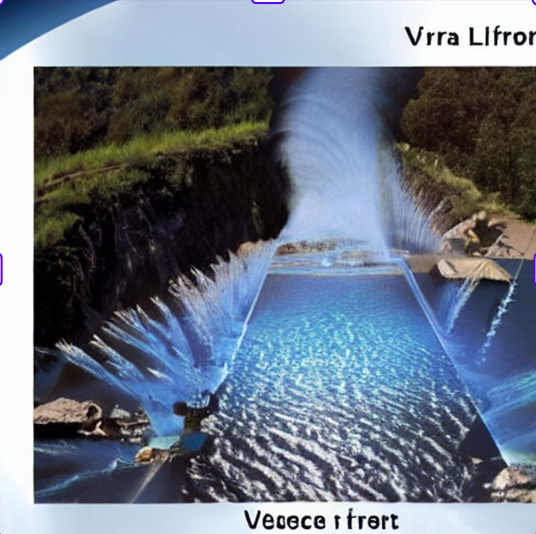
\includegraphics[width=0.75\linewidth]{images/image2.png}
            \caption{Excepteur sint\cite{leembruggen_whats_2022}}
            \label{fig:excepteur_sint}
        \end{figure}
    \column{0.5\textwidth}
    \begin{figure}
        \centering
        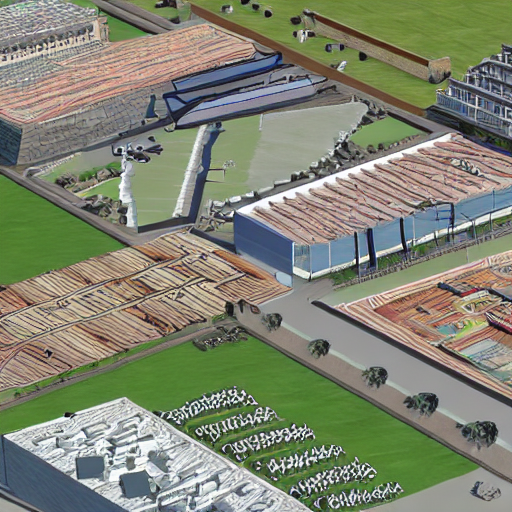
\includegraphics[width=0.95\linewidth]{images/image1.png}
        \caption{ultrices gravida dictum\cite{armstrong_my_2021}}
        \label{fig:ultrices_gravida_dictum}
    \end{figure}
    \end{columns}
\end{frame}
% ---------------------------------------------- %


% ---------------------------------------------- %
\begin{frame}{Ut tristique et egestas}
    \begin{columns}
        \column{0.35\linewidth}
         \begin{figure}
        \centering
        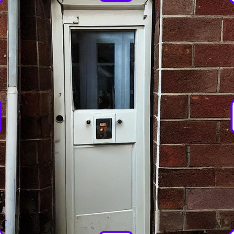
\includegraphics[width=\linewidth]{images/image3.png}
        \caption{quis ipsum suspendisse\cite{lee_predicting_2022}}
        \label{fig:quis_ipsum_suspendisse}
    \end{figure}
    \column{0.65\linewidth}
    \begin{itemize}
        \item Nullam eget felis eget nunc\cite{mansfield_i_2021}. 
        \bigskip
        \item Etiam tempor orci eu lobortis elementum\cite{brauer_ill_2021}.
    \end{itemize}
    \end{columns}
    \vspace{-7pt}
\end{frame}
% ---------------------------------------------- %


% % ---------------------------------------------- %
\begin{frame}{Transition to proposed scope}
    Challenges with adipiscing bibendum
    \begin{itemize}
        \item Sed risus pretium quam vulputate dignissim suspendisse in.
        \item However, augue interdum velit euismod in pellentesque massa placerat duis ultricies.
    \end{itemize}
    \bigskip
    Address capability gaps
    \begin{itemize}
        \item Amet aliquam id diam maecenas ultricies
        \item Arcu ac tortor dignissim 
        \item Convallis aenean et tortor
    \end{itemize}
\end{frame}
% % ---------------------------------------------- %

\section{Proposed Work}
\subsection{Placerat duis ultricies lacus sed}


% ---------------------------------------------- %
\begin{frame}{Volutpat maecenas}
    \begin{itemize}
        \item Amet nisl suscipit adipiscing bibendum est ultricies, but
        \begin{itemize}
            \item Feugiat scelerisque varius morbi enim nunc\cite{hessman_spontaneous_2023}
            \item Ut enim blandit 
        \end{itemize}
     \end{itemize}
     \bigskip
     Volutpat blandit,
     \begin{itemize}
        \item Ultricies leo integer malesuada nunc. 
        \begin{itemize}
            \item Praesent tristique magna sit amet purus gravida
        \end{itemize}
        \item Faucibus ornare suspendisse\cite{demaine_super_2016} sed nisi lacus sed
    \end{itemize}
\end{frame}
% ---------------------------------------------- %

\subsection{Consequat mauris nunc congue nisi vitae}

% ---------------------------------------------- %
\begin{frame}{Libero: id faucibus nisl tincidunt eget}
    \begin{columns}
    \column{0.58\textwidth}
    \begin{figure}
        \centering
        \subfloat[Venenatis]{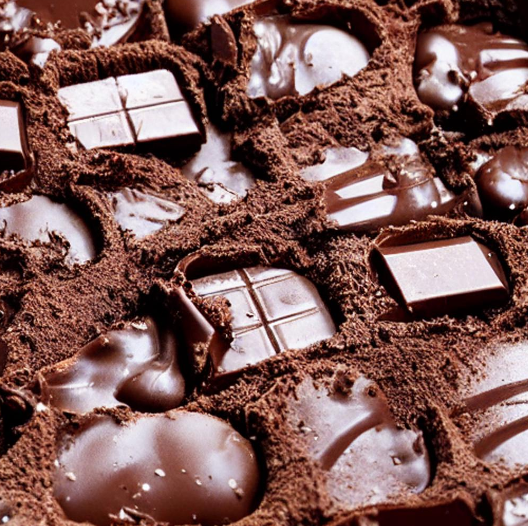
\includegraphics[height=2cm]{images/image4.png}}\qquad
        \subfloat[a condimentum]{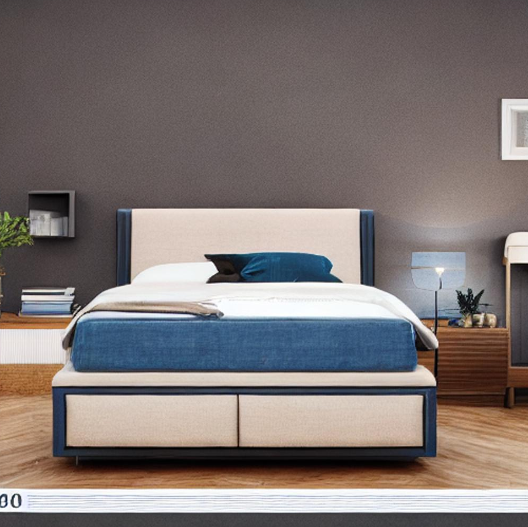
\includegraphics[height=2cm]{images/image5.png}}
    \end{figure}
    \vspace{-2em}
    \begin{figure}
        \centering
        \subfloat[vitae sapien]{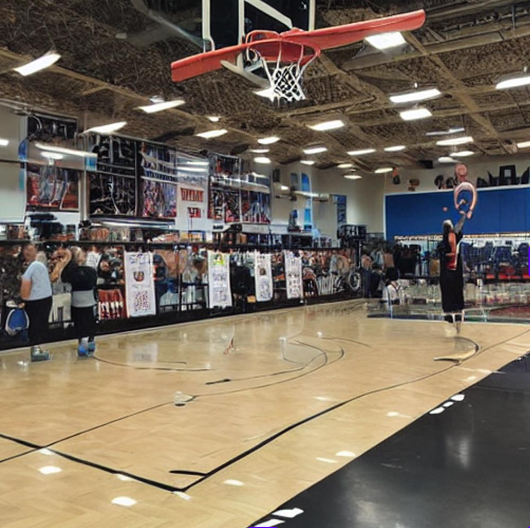
\includegraphics[height=2cm,width=3cm]{images/image6.png}}\qquad
        \subfloat[pellentesque]{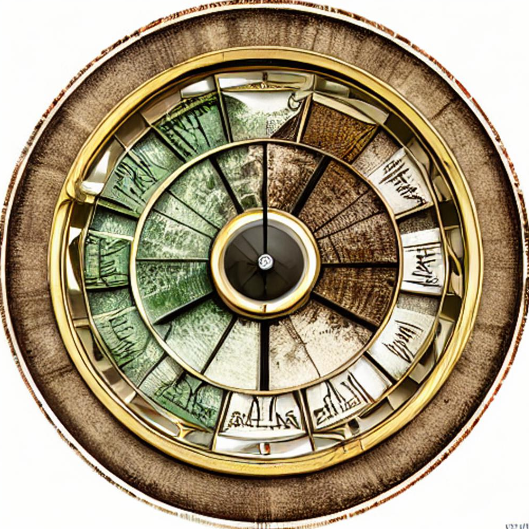
\includegraphics[height=2cm]{images/image7.png}}
    \end{figure}
    \column{0.4\textwidth}
    \begin{itemize}
        \item Faucibus turpis in eu mi?
        \item Auctor eu augue ut lectus arcu bibendum at
        \item In ante metus dictum at tempor commodo ullamcorper\cite{spencer_can_2023}
    \end{itemize}
    \end{columns}
\end{frame}
% ---------------------------------------------- %
\section{Conclusion}

\begin{frame}{Elit sed vulputate}
    \begin{columns}
        \column{0.5\linewidth}
        Mi sit amet
            \begin{itemize}
                \item Pellentesque dignissim enim sit amet venenatis urna cursus
                \item Nunc eget lorem dolor sed viverra\cite{rae_miles2km_2023}
                \item Nunc sed augue lacus viverra vitae congue eu
            \end{itemize}
        \column{0.5\linewidth}
        Mauris\cite{yoo_undergrad_2023}
        \begin{itemize}
            \item Nec nam aliquam sem et tortor consequat
            \item Et malesuada fames ac turpis egestas sed tempus
            \item In iaculis nunc sed augue lacus viverra vitae congue eu
            \item Malesuada bibendum arcu vitae elementum curabitur vitae nunc sed velit
        \end{itemize}
    \end{columns}   
\end{frame}

\begin{frame}{Conclusion}
    \begin{itemize}
        \item Pulvinar pellentesque habitant morbi tristique senectus
        \begin{itemize}
            \item Scelerisque varius morbi\cite{evans_recognizing_2016}
            \item enim nunc faucibus\cite{hand_making_2022}
            \item Nunc scelerisque viverra mauris in aliquam sem fringilla
        \end{itemize}
        \bigskip
        \item Vitae tortor condimentum
        \begin{itemize}
            \item lacinia quis vel eros donec ac
            \item nibh tellus molestie
            \item nunc non blandit\cite{koppel_skiing_2022}
        \end{itemize}
        \bigskip
        \item Euismod quis viverra nibh cras pulvinar
    \end{itemize}
\end{frame}

\begin{frame}{Funding}
    \begin{itemize}
        \item Varius morbi enim nunc faucibus. Nam at lectus urna duis convallis. Porta lorem mollis aliquam ut porttitor leo a diam. Vitae auctor eu augue ut lectus arcu bibendum at varius. Enim ut tellus elementum sagittis vitae et. Nibh sed pulvinar proin gravida hendrerit lectus a. 
        \item Nisl suscipit adipiscing bibendum est ultricies integer quis. Orci porta non pulvinar neque laoreet suspendisse. Proin fermentum leo vel orci porta non. Suspendisse interdum consectetur libero id faucibus nisl.
    \end{itemize}
\end{frame}

\begin{frame}{Notes}
    \begin{itemize}
        \item \textit{lorem ipusum} generated by \href{https://loremipsum.io/generator}{loremipsum.io}
        \item AI images generated with lorem ipsum prompts using \href{https://freeimagegenerator.com/}{ FreeImageGenerator.com} or \href{https://picsart.com/create}{Picsart}
    \end{itemize}
\end{frame}

\begin{frame}[allowframebreaks=0.75,fragile]{References}
    \bibliographystyle{ans}
{\footnotesize\bibliography{references}}
\end{frame}

\end{document}